%-----------------------------------------------
% Template para criação de resumos de projectos/dissertação
% jlopes AT fe.up.pt,   Fri Jul  3 11:08:59 2009
%-----------------------------------------------

\documentclass[9pt,a4paper]{extarticle}

%% English version: comment first, uncomment second
\usepackage[portuguese]{babel}  % Portuguese
%\usepackage[english]{babel}     % English
\usepackage{graphicx}           % images .png or .pdf w/ pdflatex OR .eps w/ latex
\usepackage{times}              % use Times type-1 fonts
\usepackage[utf8]{inputenc}     % 8 bits using UTF-8
\usepackage{url}                % URLs
\usepackage{multicol}           % twocolumn, etc
\usepackage{float}              % improve figures & tables floating
\usepackage[tableposition=top]{caption} % captions
%% English version: comment first (maybe)
\usepackage{indentfirst}        % portuguese standard for paragraphs
%\usepackage{parskip}

%% page layout
\usepackage[a4paper,margin=30mm,noheadfoot]{geometry}

%% space between columns
\columnsep 12mm

%% headers & footers
\pagestyle{empty}

%% figure & table caption
\captionsetup{figurename=Fig.,tablename=Tab.,labelsep=endash,font=bf,skip=.5\baselineskip}

%% heading
\makeatletter
\renewcommand*{\@seccntformat}[1]{%
  \csname the#1\endcsname.\quad
}
\makeatother

%% avoid widows and orphans
\clubpenalty=300
\widowpenalty=300

\begin{document}

\title{\vspace*{-8mm}\textbf{\textsc{Test Automation in Continuous Integration for Hardware Validation}}}
\author{\emph{Pedro Dias Faria}\\[2mm]
\small{Dissertação realizada sob a orientação do \emph{Prof.\ Rui Filipe Lima Maranhão de Abreu}}\\
\small{na \emph{Synopsys Portugal Lda}}}
\date{}
\maketitle
%no page number 
\thispagestyle{empty}

\vspace*{-4mm}\noindent\rule{\textwidth}{0.4pt}\vspace*{4mm}

\begin{multicols}{2}

\section{Motivação}\label{sec:motiva}

O processo de validação de hardware está diretamente relacionado com a verificação se as diferentes configurações dos clientes serão cumpridas. Como tal, o processo de validação pode tornar-se num processo subjetivo, uma vez que envolve a avaliação de como o comportamento do hardware irá atuar nas mais diversas aplicações e condições. O processo normalmente consiste em atividades que incluem modelagem de sistemas, prototipagem e avaliação pelo utilizador\cite{TroyScott}\cite{Puri-Jobi2015}.

Com esta dissertação, ajudamos a construir um ambiente de integração contínua para a validação de hardware, desenvolvendo um plugin de Jenkins em forma de \textit{dashboard}, com o objectivo de ajudar as equipas de R\&D da Synopsys no processo de prototipagem do hardware.

\section{Ojectivos}\label{sec:goals}
A subjetividade do processo de validação em qualquer tipo de desenvolvimento de software requer o uso de algum tipo de estrutura e categorização de dados. Isto pode ajudar a um acesso mais fácil na resolução de falhas no desenvolvimento.

Com a nossa solução, a produtividade nas equipes de desenvolvimento deverá aumentar, tendo esta informação exibida de forma simplificada, precisa e direta.
Para sua validação, o sistema teve que ser implementado num projeto real e recolhido feedback da equipa para se perceber se o valor gerado é visível.

Os objetivos da dissertação são:

\begin{itemize}
\item Definir uma estrutura automática de gestão de testes para a validação de Hardware;
\item Definir técnicas para categorização e gestão dos resultados dos testes de validação de Hardware;
\item Desenvolver uma aplicação web de suporte ao sistema automático de testes;
\item Testar a aplicação e validar a sua utilidade.
\end{itemize}

\section{Descrição do Trabalho}\label{sec:work}

Uma vez que a Synopsys já tinha configurado o servidor de CI em Jenkins, foi decidido desenvolver um Plugin para esta ferramenta. Temos também a vantagem de Jenkins ser muito costumizável, com centenas de \textit{extension points} e plugins disponíveis para suportar as nossas necessidades~\cite{kn:Jenkins}.

\subsection{Casos de Uso}\label{sc:usecases}

Tendo em consideração a organização dos projetos R\&D no Jenkins, foi discutido com a equipa colaboradora que a melhor opção era desenvolver o Dashboard como um \textit{View plugin}, implementando a classe \textit{ViewGroup}, com o propósito de agregar diferentes Views dentro da mesma.

No diagrama de Casos de Uso da figura~\ref{fig:usecases} estão representadas as ações que um utilizador pode executar para exibir o nosso Dashboard no ambiente do Jenkins.

\newcommand{\code}{\texttt}

\begin{figure}[H]
\centerline{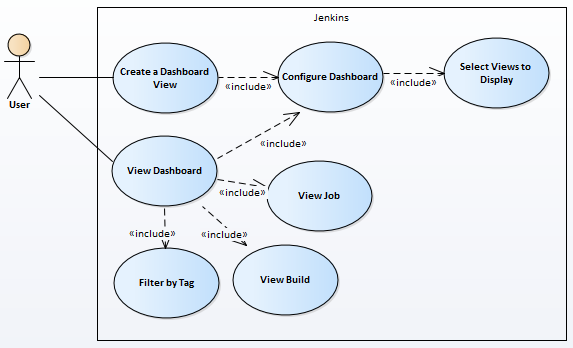
\includegraphics[scale=.4]{figures/usecases.png}}
\caption{Diagrama de Casos de Uso do plugin}  
\label{fig:usecases}
\end{figure}

O plugin foi desenhado para ser tão simples como criar uma nova \textit{View} dentro da ferramenta, selecionando quais as outras Views a serem exibidas. Depois, o utilizador pode alterar livremente a sua configuração, ou seja, adicionar, remover ou alterar quais \textit{Views} a serem exibidas.

\subsection{Jenkins Plugin - Filtered Dashboard View}\label{sc:dashboard}

\subsubsection{Mission Control Plugin}\label{mission_plugin}

Sabendo que queremos criar um Dashboard, encontramos o \textit{Mission Control Plugin}~\cite{jkns:missionC}, que tem praticamente toda a base para desenvolver, uma \textit{dashboard View} completa contendo:

\begin{itemize}
\item Exibição dos estados dos \textit{Jobs};
\item Histórico e filas de \textit{Builds};
\item Extende um objeto \textit{View}, que poderá ser adicionado ao \textit{dashboard} principal.
\end{itemize}

Apesar de ser um ponto de partida, precisava ser moldado e adaptado às nossas necessidades.

\subsubsection{Metadata Plugin}\label{metadata_plugin}

Considerando que um dos requisitos é filtrar os dados exibidos com as informações de cada configuração de teste, e uma vez que Jenkins tem a possibilidade de armazenar informações sobre cada um de seus items em formato XML, então também poderia ser armazenado algum tipo de \textit{metadata}.

Para facilitar isso, usamos o \textit{extension point} que o \textit{Metadata Plugin}~\cite{jkns:metadata} fornece, em conjunto com a API Jenkins, para aplicar filtros relevantes em cada \textit{Job} para uma análise mais fácil dessas informações das configurações.

Esta \textit{Metadata} pode ser aplicada a \textit{Jobs} simplesmente através do menu de customização, no qual aplicará a todas as \textit{Builds} futuras.

Ou alternativamente, automatizar o processo chamando simplesmente um comando CLI de \textit{post-build}, fornecido pelo mesmo plugin.

\subsection{Server Side Implementation Design}\label{sc:implementationDesign}

Compreender como o \textit{back-end} em Java interage com Jenkins e como os projetos foram organizados em \textit{Views}, definimos uma estratégia de \textit{Top-down} para obter e analisar as informações dos nossos items de interesse.
Isto significa que tivemos que processar \textit{View} a \textit{View} como projetos individuais para relacionar os seus items filho no nosso Dashboard, como demonstrado na figura~\ref{fig:dashboardDiagram}.

\begin{figure}[H]
\centerline{\includegraphics[scale=0.2]{figures/dashboardDiagram}}
\caption{Diagrama de abordagem \textit{Top-down}}  
\label{fig:dashboardDiagram}
\end{figure}

Finalmente, a adição de \textit{Tags} para filtrar as informações é a principal característica do nosso Dashboard. Este conceito ajuda o rastreamento de cada configuração, com o requisito mínimo de adicionar ou modificar essas classificações dos \textit{Jobs} no \textit{building process}.

Este design permite uma estrutura totalmente escalável, uma vez que não tem limitações no número de \textit{Views} associados ao Dashboard, nem dos seus \textit{Jobs} e \textit{Builds}. Também pode ser extensível para armazenar mais informações em cada uma das suas classes personalizadas, para cálculo de métricas e indicadores adicionais no futuro, se pretendido. Todas estas informações só dependem da API do Jenkins e do que esta suporta.

\subsection{Front-End Implementation Design}\label{sc:frontend}

Para a estrutura da organização da inforação, no \textit{front-end} do Dashboard, baseámo-nos nos mesmos scripts do \textit{ Mission Control Plugin}, descritos na seção~\ref{mission_plugin}, juntamente com várias bibliotecas e \textit{Web App frameworks} comuns como Javascript, JQuery e Bootstrap, todos processados em Apache Jelly, um \textit{engine} de processamento de scripts baseados em Java e XML que permite que a UI do Jenkins seja estendida.

Como os dados exportados para a API já estão bem estruturados, o processo de apresentação foi concluído com facilidade, exigindo apenas uma maneira de exibir a \textit{View} de um projeto com uma vista intuitiva.

Para completar o acima mencionado, foi decidido exibir cada \textit{Job} dentro do projeto como uma coluna numa tabela, sendo cada célula da linha as suas \textit{Builds} organizadas em ordem cronológica decrescente. Cada célula tem suas \textit{Tags} associadas para uma referência rápida das configurações utilizadas na respectiva \textit{Build}.

\section{Conclusões}\label{sec:conclui}

No final deste projeto fomos capazes de desenvolver com sucesso o plugin de Dashboard pretendido~\cite{jksn:myplugin}.

Embora reduzindo algumas das características esperadas no início do projeto, como exibir métricas sobre o processo de validação de hardware devido a restrições de tempo entre o fim do desenvolvimento e testes do Plugin, acreditamos que irá ajudar as equipas de desenvolvimento a manter o rastreamento dos seus projectos de forma mais simples e precisa.

%%English version: comment first, uncomment second
\bibliographystyle{unsrt-pt}  % numeric, unsorted refs
%\bibliographystyle{unsrt}  % numeric, unsorted refs
\bibliography{refs}

\end{multicols}

\end{document}
